\documentclass{mpaper}

\usepackage{hyperref}
\usepackage{rotating}
\usepackage{booktabs}
\usepackage{pifont}
\newcommand{\cmark}{\ding{51}}%
\newcommand{\xmark}{\ding{55}}%
\usepackage{enumitem}
\usepackage{gensymb}


\begin{document}

\title{TactiHelm: A Vibrotactile Helmet for Cycling Safety}
\author{Lewis Trundle}
\matricnum{2469635t}

\maketitle

\begin{abstract}
Despite significant advancements in motor-vehicle safety, such progress has not yet extended to cyclists, who continue to suffer thousands of fatal injuries annually worldwide, often due to collisions with road vehicles approaching from behind. Typical cyclist safety technologies rely on visual and auditory alerts for approaching vehicles, however, these sensory channels are often already in use whilst cycling. Vibrotactile stimulation offers a suitable alternative. Despite much prior work investigating methods for delivering vibration stimuli, few have explored how this can be used for cycling safety. In response, we continue previous work to develop TactiHelm: a vibrotactile, helmet-based, hazard-notification system, which can effectively warn a cyclist of vehicles approaching from behind. We combined a commercial bike radar with a modified cycling helmet to detect and convey distance information for approaching vehicles, using tactile actuators placed along the sagittal midline of the helmet. We conducted a study investigating how distance information can be encoded using the pattern and duration of a vibrotactile cue. Results showed that encoding schemes which vary the number of cue deliveries, led to a significantly higher percentage of correctly interpreted cues. Furthermore, participants preferred tactile patterns which create a sensation of movement across the scalp. TactiHelm was shown to be effective in real life, with commuter cyclists reporting its usefulness in portraying the approach of a vehicle, without consuming their sight or hearing, making them feel safer.
\end{abstract}

\section{Introduction}
Each year, road-traffic accidents account for 1.35 million deaths worldwide, with cyclists comprising 41,000 of these fatalities \cite{world2018global}. The economic burden associated with road accidents in the EU alone is estimated to amount to 236 billion euros annually \cite{costoftransport}. Despite the EU achieving an average annual reduction of 3\% in motor vehicle related fatalities between 2010 and 2018, the fatality rate for cyclists remained the same across that period \cite{adminaite2020safe} - emphasising the lack of attention towards cyclists regarding road safety.

One of the primary causes of cyclist fatalities is collisions with motorised vehicles \cite{BIL20101632}, with 78\% of cyclist fatalities in the EU due to bicycle-to-vehicle collisions \cite{adminaite2015making}. Although a collision with another vehicle may occur from any angle, situations where the offending vehicle crashes into the cyclist from behind cause the largest proportion of fatalities of all crash directions \cite{BIL20101632}. Despite a large body of research investigating how cyclist safety can be improved using safety systems implemented within other road vehicles \cite{scholliers2014potential, SILLA2017134, cieslik2019improving, 7929602, 10.1145/3434770.3459732}, few studies have explored how cyclist safety can be improved from the perspective of the cyclist \cite{10.1145/3490099.3511127, STROHAEKER2022151}. 

Studies investigating the cognitive demand of cycling has shown that novice cyclists often struggle to accomplish the cognitive tasks which are necessary for traffic safety, such as looking for traffic and identifying the type of intersection \cite{https://doi.org/10.1002/acp.2350050205}. To aid cyclists, safety technology such as rear-view bike radars \cite{garminradar} help reduce cognitive load, by delivering warning messages about approaching vehicles both visually and audibly, without the cyclist having to shoulder check, which takes their eyes of the road ahead. However, auditory messages have been shown to be difficult to understand in noisy environments \cite{noisyenv} and in situations such as when the cyclist is listening to music, which many admit to doing \cite{DEWAARD2011626}.

A possible alternative message modality is vibrotactile stimulation. Many previous works have explored different methods for delivering vibrational stimuli, utilising belts \cite{10.1145/2449396.2449450, 10.1145/1060581.1060585}, vests \cite{10.1145/2556288.2557404}, and even bicycles themselves \cite{10.1145/2371574.2371631, 10.1145/3290605.3300850}. However, an unexplored area is the potential of the helmet. Few studies have explored how vibrotactile stimuli can be used in helmets \cite{10.1007/978-3-642-39802-5_3, yamauchi2020vibro} and even fewer have investigated how this can be applied in the context of cycling \cite{krauss2021head}.

In this paper, we continue previous work from Vo et al. \cite{10.1145/3411763.3451580}, to develop TactiHelm: a vibrotactile, helmet-based, hazard-notification system, which can effectively warn a cyclist of vehicles approaching from behind. The system utilises a commercial bike radar to detect the distance and speed of approaching vehicles from behind the cyclist, which is subsequently conveyed to them using vibrotactile feedback delivered to the head. The TactiHelm system aims to improve cycling safety, by alerting the cyclist of potential collisions through their tactile sensory channel, as opposed to potentially distracting visual or auditory methods - helping reduce the cognitive demand required of the cyclist. Through development of this system, we define and investigate two primary research questions:

\textbf{RQ1: How can meaningful information about an approaching vehicle be encoded using vibrotactile feedback delivered from a helmet?} The amount of information that a vibrotactile display can effectively convey is limited by the number of perceptually distinguishable levels afforded by the parameters of the system \cite{guidelines}. This is subsequently limited by the on-body location of where these stimuli are delivered. Therefore, we consider how information about an approaching vehicle, such as its distance and speed, can be quantised and represented using vibrotactile stimulation. Furthermore, we investigate what parameters of a helmet-based vibrotactile display, are most suitable for encoding this information. \label{sec:rq1}

\textbf{RQ2: Is our developed TactiHelm system effective for warning cyclists in real-world scenarios?} For our system to be effective, people must be able to accurately perceive and interpret our defined vibrotactile cues on their scalp whilst cycling. Furthermore, these cues must be meaningful, and should help improve perceived safety. Therefore, we assess TactiHelm using a real-world user study, where participants evaluate the system in realistic traffic conditions. \label{sec:rq2}



\section{Background}
Little literature exists on the use of vibrotactile feedback for cycling, and of the existing corpus, few relate to the problem of cyclist safety. To address this issue, we survey four broad areas of research, and combine the insights we gather to inform our approach to developing TactiHelm. We first examine existing literature regarding hazard notification systems for cyclist safety. We then explore how different feedback modalities have been used in cycling. Finally, we review ways in which vibrotactile stimuli can be used to encode information, and how this can be applied to the head.

\subsection{Hazard Notification for Cyclist Safety}
Hazard notification systems were first explored by Horowitz and Dingus \cite{doi:10.1177/154193129203601320}, who proposed ideas, such as varying the warning intensity based off the detected collision time, and using different signal modalities to convey various warning severities. These concepts have been used often in later research, such as by Langer and Jochem \cite{566402} and Huang et al. \cite{1307429} who combined radar and vision technologies to detect and classify road vehicles ahead of the car, with up to 97\% accuracy, showing that even relatively older vehicle detection systems are highly reliable.

Jenkins et al. \cite{7929602} showed how cyclist detection could be implemented using Bicycle to Vehicle communication systems. By outfitting cyclists with a human-machine interface (HMI), they were able to receive basic safety messages, delivered using multimodal audio and haptic cues, from a smartphone speaker and attachable handlebar grips \cite{smartgrips}. These safety messages were categorised into five levels, describing recommended actions to the cyclist. Lujic et al. \cite{10.1145/3434770.3459732} furthers this idea, by creating an Edge network around a city which would detect when a pedestrian or cyclist entered a vehicles' blind spot, sending a visual and auditory warning to driver's mobile device in real-time using 5G. These papers showcase the potential ways in which feedback modalities can be used to improve cyclist safety. Furthermore, they highlight potential warning messages which could be used in our system. These don't necessarily convey information about the potential threat, but rather they recommend actions to avoid danger.

These warning systems are examples of Intelligent Transport Systems (ITSs) - a series of technologies which aim to improve the safety of transportation \cite{its}. Although few address how the safety of vulnerable road users (VRUs), such as cyclists, can be improved \cite{Scholliers2017}, of those which do, a quantitative safety impact assessment found that vehicles which contain a dedicated VRU detection system would have the greatest impact for cyclists \cite{SILLA2017134}. However, despite their potential for improving cyclist safety, studies have shown that pre-existing attitudes and perceptions affect the acceptance of such systems. One such study from Angelis et al. \cite{de2017negative}, found that drivers who already express a negative representation of cyclists are more unlikely to use a cyclist detection system, compared to those who do not. This is further explored by Berge et al. \cite{berge2022cyclists} who studied acceptance from the perspective of the cyclist. Through questionnaires and interviews, the authors found that cyclists were worried about using technologies, such as HMIs, as they believed such technologies would force them to take responsibility over safety critical situations, regardless of whether or not it was their fault. This finding motivates the need to further study cyclists' beliefs and attitudes towards cycling safety, to ensure that a technology such as TactiHelm would be accepted.


\subsection{Feedback Modalities in Cycling}
Wolfe et al. \cite{wolfe2016distracted} investigated different types of distractions which cyclists commonly face, finding that auditory distractions were most common, followed shortly by visual ones. These distractions commonly occur from interaction with a mobile device, which studies have found to increase the risk of crashing whilst cycling \cite{mwakalonge2014distracted, doi:10.1080/19439962.2019.1591559}. With over half a surveyed population admitting to using their mobile device on every trip \cite{GOLDENBELD20121}, there have been calls to put legislation in place to prevent the use of smartphones whilst cycling \cite{banphoneuse}. While some studies investigate ways to improve smartphone interaction whilst cycling to reduce distraction \cite{10.1145/3544548.3580971, 10.1145/3152832.3152871} other approaches have investigated alternative interaction modalities, which don’t consume the cyclists visual senses.

Pielot et al. showed how vibrotactile stimulation can be effective in improving cyclists' visual focus, by developing Tacticycle - a bicycle with a set of directional cues encoded by the relative intensity across both handlebars \cite{10.1145/2371574.2371631}. Although the authors remark that the navigational routes used in their study were simple, no participants reported losing orientation, and positively described the ease of interpreting the vibrotactile cues, with minimal cognitive effort. Steltenpohl and Bouwer support these findings using Vibrobelt - a vibrotactile belt also developed to aid navigation while cycling \cite{10.1145/2449396.2449450}. Through analysis of visual focus and spatial knowledge acquisition, they found that Vibrobelt increased participants ability to recall images from the route; however, they were generally slower at navigating. These studies showed that vibrotactile feedback is an effective way of communicating information without decreasing the cyclists' visual focus - an important aspect of cycling.

This concept of utilising different sensory channels to convey information is studied by Wickens \cite{wickens1984processing} and Wickens and Liu \cite{doi:10.1177/001872088803000505}, who explored \textit{Multiple Resource Theory} - a model of human information processing which predicts that attention is a limited cognitive resource that can be allocated across different tasks and modalities. The model implies that multiple sensory channels can be used simultaneously, without impairing the attention of an individual, within their cognitive capacity. Seeking to take advantage of this concept, Wickens suggests that tasks can be configured to utilise these multiple sensory channels - exploiting our information-processing capabilities.

Previous studies have explored this idea further, by comparing the effectiveness of unimodal and multimodal warning messages for cyclists. Strohaeker et al. \cite{STROHAEKER2022151} compared auditory and vibrotactile warnings. They found that auditory warnings were more effective for decreasing participants response time to potential collisions, but vibrotactile warnings were still effective for a system which does not require urgent reactions from the cyclist. However, a study conducted by Peeters et al. \cite{peeters2019vibrotactile} found that vibrotactile signals were not only perceivable during diverse levels of physical effort, but that cyclists' reaction time to stimuli shortened as they cycled with greater effort, acknowledging the potential of utilising tactile feedback for cycling. Matviienko et al. \cite{10.1145/3290605.3300850, 10.1145/3229434.3229479} expanded upon this research by comparing the delivery of navigational instructions to child cyclists using visual, auditory, and vibrotactile feedback. Their results showed that when instructions were delivered multimodally, cue interpretation accuracy increased and cyclists showed a shorter reaction time to potential dangers. These findings are backed by Sawitzky et al. \cite{10.1145/3490099.3511127, mti6010003} who similarly compared the combination of different awareness message modalities for cyclists, finding that a multimodal combination of visual messages and auditory icons was preferred by participants. 
Although these studies clearly outline the potential benefits of providing feedback multimodally, we keep our TactiHelm system restricted to only unimodal vibrotactile feedback, so that we may thoroughly assess the impact this has on cyclists' perceived safety and focus.

Despite auditory and vibrotactile modalities having the potential to aid visual feedback, they each have disadvantages. Waard et al. \cite{DEWAARD2011626} found that 68\% of auditory cues were missed when participants were listing to music, an act which many admit to doing. Although this could be mitigated by wearing bone conducting headphones \cite{wolfe2016distracted}, May and Walker \cite{may2017effects} found that their usage worsened participants ability to localise critical environment sounds. Erdei et al. \cite{erdei2020comparing, doi:10.1080/15389588.2021.1985113} reported that perception of vibrotactile signals worsen when cycling over surfaces which cause haptic interference. However, they suggested this could be overcome by adjusting how the stimuli was delivered to the cyclist. This motivates our decision to deliver vibrotactile stimuli through the cycling helmet, as this remains in-contact with the rider at all points of the journey and haptic interference received from the terrain dissipates the further it travels \cite{9415164}, with the helmet being one of the furthest points of contact away from the source of interference. Therefore, delivering tactile stimuli from the helmet to the scalp allows for greater perception.

\subsection{Using Vibrations to Encode Distance}
Parameters to encode information is studied by van Erp, who explores spatial and temporal effects of vibrotactile stimuli \cite{guidelines}. The paper serves as a set guidelines for implementing a vibrotactile system and suggests that a vibrotactile display affords five adjustable parameters: the location, timing, frequency, amplitude, and waveform of a vibration. How these parameters can be used is described by Brewster and Brown \cite{10.5555/976310.976313}, who introduce \textit{Tactons} - structured, abstract messages, whose meaning is encoded using the parameters of tactile perception. The authors expand on the parameters suggested by van Erp, explicitly describing how temporal characteristics of a vibration, such as rhythm and duration can be used.

Previous studies have investigated how these parameters can be used to encode distance. van Erp et al. \cite{10.1145/1060581.1060585} and Straub et al. \cite{5326374} both performed similar studies, investigating the effectiveness of different distance encoding schemes to aid navigation for pedestrians. Both studies used different combinations of rhythm, duration, intensity, and frequency to encode distance, finding that access to distance information did not aid the navigational performance of participants. However, the authors from both studies admit this is likely attributable to the confounding of parameters in their defined schemes.

These inconclusive findings identified a need to further explore how distance could be encoded using temporal aspects of vibrotactile stimulation, something which the skin is sensitive to \cite{doi:10.1068/p5014}. McDaniel et al. \cite{10.1145/1520340.1520718} utilised tactile rhythms to convey four different short-range distances, to the blind. This was done by decreasing the delay between vibration pulses as the distance decreased. The experiment proved effective and showed that given a small training period, users were able to effectively identify different tactile rhythms and associate them with their respective distances.

Pielot et al. \cite{10.1145/1753326.1753581} further studied distance encodings, comparing rhythm, duration, and intensity based schemes, for a fast-paced 3D multiplayer game. Participants found the rhythm-based scheme the easiest to judge distance. Furthermore, they proved it was possible to accurately perceive and interpret vibrotactile signals in an environment with high cognitive demand, similar to a task such as cycling in our context.

Asif et al. \cite{10.1145/1868914.1868923} further studied how rhythm can be used to encode distance, comparing three rhythm-based schemes: rhythm only, rhythm and intensity, and rhythm and duration. These schemes were used in-vehicle, to indicate four different categories of distance until an approaching turn. The results found that the combination of rhythm and duration (where the pulse duration stayed the same but the number of pulses decreased as the distance decreased) was the easiest for participants to learn and led to the smallest amount of navigational mistakes. 

This finding motivated Prasad et al. \cite{10.1145/2556288.2557404} to develop HaptiMoto - a wearable vest which provides vibrotactile feedback regarding upcoming turns for motorcyclists. Through a user study, they were able to prove that the rhythm and duration coding scheme for distance, was effective at providing navigational instructions to motorcyclists. This paper highlights the effectiveness of using a rhythm and duration to encode different distances. Additionally, this study was performed at low speeds of below 25 mph, suggesting that these results may be similarly applied to our cyclist demographic.



\subsection{Vibrotactile Stimulation on the Head}
Gilliland and Schlegel \cite{doi:10.1177/001872089403600410} studied the spatial acuity of the head, investigating how various configurations of 4 to 12 tactile actuators, placed across the coronal plane of the head (from ear to ear), affected localisation ability. They found that optimal tactile detection and localization accuracy occurred when using six actuators - with a 93\% accuracy. More than this, and both the accuracy and reaction time worsened. 

Myles and Kalb \cite{headguidelines} explored how tactile perception varied across different regions of the head, using various configurations of eight actuators. They found that the scalp was the least sensitive loci on the head, whereas, the regions around the axial plane of the head (namely the forehead, occipital, and temple regions) were the most sensitive. These different regions can be seen in Figure \ref{fig:head-regions}. In subsequent research, Myles et al. \cite{MYLES2015177} determined that the density of hair on the head only minimally impacts tactile perception. Furthermore, this effect is confined to only the regions of the head which are the least sensitive.

de Jesus Oliveira et al. \cite{7463147} continued Myles and Kalb's work, by comparing the spatial resolution of the identified sensitive head regions around the axial plane. Although they found that the forehead was the most accurate region for spatial discrimination of vibrotactile stimuli, they also showed that the centre of the occipital region had high precision, which decreased as the distance from the head midline increased. This phenomenon was named the \textit{Midline Effect}, and had previously been indirectly reported on by van Erp \cite{1406917}. He proposing various hypotheses for the effect, that include the body's midline serving as an anchor point to assist in absolute localization, or that the central nervous system possesses specific characteristics for processing stimuli. Regardless of the reason, de Jesus Oliveira et al. suggests further research is needed investigating the effect - highlighting the need to investigate how tactile perception differs between regions of the head across the sagittal plane.

Few studies have explored how vibrotactile feedback can be utilised in a helmet. Bertram et al. introduced the Tactile Helmet \cite{10.1007/978-3-642-39802-5_3} which communicated the distance of a detected object to a pedestrian wearer using the intensity of a vibration. Yamauchi and Suzuki \cite{yamauchi2020vibro} extended this by demonstrating how such a helmet could be used for hazard notification for motorcyclists. The direction of a hazard corresponded to the location of a vibration around the axial plane of the head, whereas the vibration strength corresponded to the level of risk. They showed that the use of four directions and three levels of intensity was effective at notifying a wearer of an approaching hazard, even in winds of up to 100km/h.

However, in the context of cycling, only two studies to the best of our knowledge have investigated how vibrotactile stimulation around the head can be used. Krau{\ss} et al. \cite{krauss2021head} developed a navigational headband which vibrated on the wearers head in the direction of travel - using 12 actuators for a spatial resolution of 30\degree{}. They demonstrated that vibrotactile stimulation could be used on the head whilst cycling, without any reported discomfort or distraction. Similarly Vo et al. introduces the TactiHelm helmet \cite{10.1145/3411763.3451580} - a cycling helmet aimed to inform cyclists to potential collisions. Direction was conveyed using one of four tactile actuators in the cardinal directions and two distance levels were encoded using two distinct tactile cues. They showed that cyclists were able to accurately identify the proximity and direction from a cue 91\% and 85\% of the time respectively. This highlighted the potential of TactiHelm as a hazard notification system for cyclists, and it is from this work which this paper is inspired to continue development of such a system.


\section{Exploratory Survey}\label{sec:survey}
To identify the requirements of a hazard notification system such as TactiHelm, an online survey was conducted to understand cyclists' attitudes and behaviours towards safety while cycling. The survey used a mixture of open response, Likert scale, and multiple choice questions to explore topics such as use of safety equipment and techniques and causes of injuries. It was distributed to various cycling groups around Glasgow. We emphasised that we did not intend to judge any participants' answers on their safety or legality - instead we only wish to gather insights for use for the project.

The survey was answered by 110 respondents, aged 16-24 (14.55\%), 25-34 (10.91\%), 35-44 (11.82\%), 45-54 (31.82\%), 55-64 (24.55\%) and 65+ (5.45\%) years old. Participants identified as 61.82\% male, 37.27\% female, and 0.91\% other. Roughly 90\% of respondents were from Scotland, with the majority from Glasgow. These demographic data were collected as studies have shown that the risk and severity of cyclist injuries vary depending on factors such as roadway characteristics and demographic group \cite{BEHNOOD201735}.

90\% of respondents answered saying they cycle more than one hour a week, with 42.73\% cycling 7+ hours a week. Respondents equally cycled on city roads (30.37\%), cycle paths (29.63\%), and country roads (28.15\%), with the remaining 11.85\% cycling in other environments. Notably, 72.73\% of respondents answered that they had suffered some kind of injury while cycling - 60\% a minor injury and 12.73\% a major injury. Reasons for injury varied, from slipping on wet and uneven roads, to colliding with another road vehicle.

Over 80\% stated that they regularly wear a helmet. When asked for reasons for not wearing a helmet, a variety of responses were given, with the most common being that they are not available when hiring a bike. Some respondents answered that they did not believe helmets to be useful in certain scenarios, \textit{“Helmets are designed to prevent injury at relatively low speeds, speeds which are comfortably exceeded by adult cyclists of even moderate fitness. I believe the effectiveness of helmets to prevent injury is grossly overstated”} [P13]. However, multiple studies conducted on the effectiveness of bicycle helmets \cite{10.1093/ije/dyw153, HOYE201885, HOYE2018239, buth2023effectiveness} have found that regardless of the crash severity, helmets can help reduce the severity of head injuries by 48\% \cite{HOYE201885}.

When asked about safety technology, the most common equipment following from a helmet were cycle lights (87.27\%), reflective gear (64.54\%), and bike computers or mounted smartphones (60.90\%). Of nine respondents who stated they had a bike radar, all of them said they had a Garmin radar. When asked to comment on its usefulness they all expressed that they benefit from being more aware of vehicles behind them; however, a common disadvantage is its high cost.

Participants were asked to freely respond with the challenges they face which makes cycling feel unsafe. Categorising the responses, the most common ones were \textit{“close passes from cars”} (38.18\%), followed shortly by \textit{"poor cycling infrastructure”} (34.54\%).

Finally, participants were provided with a brief description of TactiHelm and were invited to comment on its usefulness for cycling. Respondents thought the concept could be useful, but were worried that it may be distracting - expressing concern that it may remain vibrating at all times while a vehicle is detected. These comments are useful in understanding users pre-conceived notions and worries as to how such as system may operate, and help shed light on specific problems which should be addressed in TactiHelm.


\section{TactiHelm}
\subsection{The TactiHelm System}\label{sec:tactihelm-system}
The TactiHelm system is composed of three primary components: the helmet, a Garmin bike radar, and the controller application on a mobile device, as seen in Figure \ref{fig:setup}. The TactiHelm helmet builds on previous work from Vo et al. \cite{10.1145/3411763.3451580}, and can be seen in Figure \ref{fig:helmet}. The inside lining of the helmet is equipped with 10mm diameter, three volt ERM coin cell tactile actuators. The intensity of these are controlled by PWM signals from 0 to 3V generated by an Arduino Uno micro-controller \cite{arduinouno}, which is subsequently powered by a 9V battery. PWM varies the voltage to the actuator in such a way that it is represented as an analogue signal - simultaneously effecting the frequency and amplitude of the signal wave \cite{kart2001pulse}. Therefore, the term \textit{'intensity'} refers to the combined effects of vibration frequency and amplitude. The circuit is also equipped with an HC-06 Bluetooth Module \cite{hc06}, which can connect to a mobile device using Bluetooth Classic, allowing for remote control over the actuators.

\begin{figure}[ht]
    \centering
    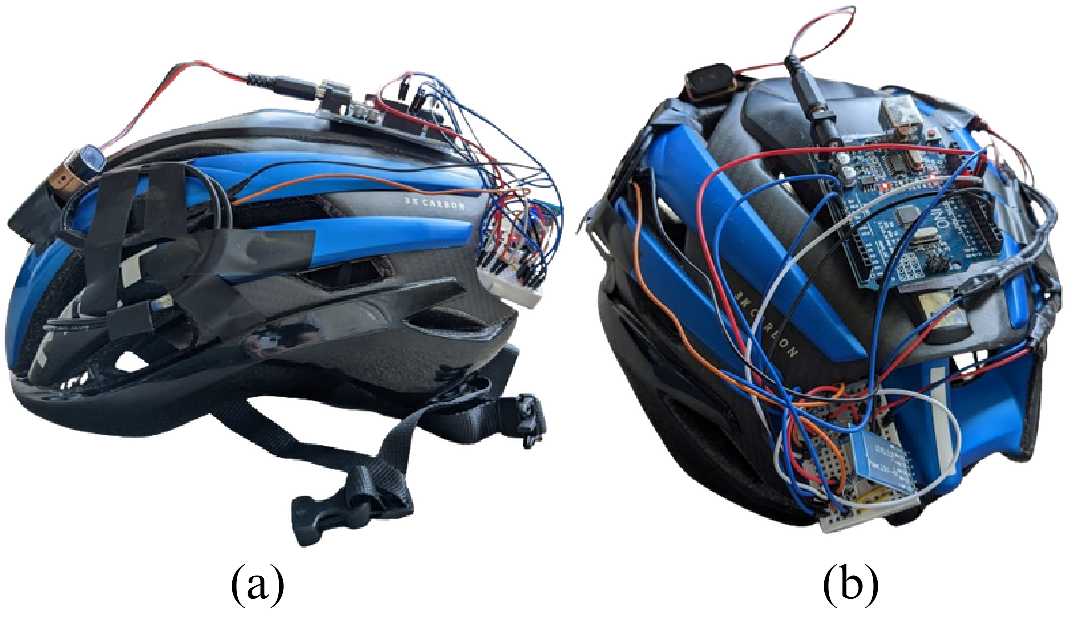
\includegraphics[width=0.44\textwidth]{images/helmet-views.pdf}
    \caption{The developed TactiHelm helmet: (a) side-view, (b) rear-view.}
    \label{fig:helmet}
\end{figure}


A custom Android application, known as the \textit{controller}, was developed to allow communication between the bike radar and Arduino. The controller acts as a pipeline between the two devices: parsing information received from the radar into the relevant instructions for the Arduino to deliver the specified stimulus. Furthermore, the application provides manual control over the actuators, giving the researchers precise control over the location, intensity, and further attributes of delivered stimuli.

The bike radar used in this project was the Garmin Varia RTL515 \cite{garminradar}. Designed to attach to the back of a bicycle, the radar can detect vehicles within a 140-metre range and offers a 220\degree{} viewing angle. This allows for complete detection of vehicles approaching from behind, extending beyond the cyclist's standard peripheral vision \cite{Spector1990VisualFields}. The radar detects approaching vehicles’ distance and speed, and sends this to the controller application using Bluetooth Low Energy. These are then used to calculate the following distance of the closest approaching vehicle. 

\begin{figure}[ht]
    \centering
    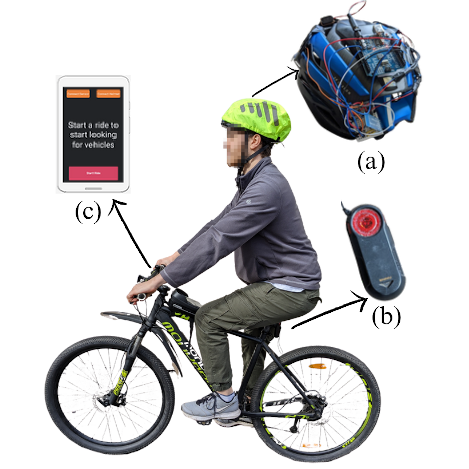
\includegraphics[width=0.44\textwidth]{dissertation/images/TactiHelm Setup.pdf}
    \caption{A commuter cyclist equipped with (a) TactiHelm helmet with attached rain cover (b) Garmin Varia RTL515 bike radar, and (c) a mobile device hosting the controller application.}
    \label{fig:setup}
\end{figure}

\subsection{Alerting Using Following Distance}
The following distance is a commonly used metric in road-safety: defined as the time it would take an approaching vehicle behind a cyclist to reach their location if they were to suddenly stop \cite{followdistancedef}. The exact recommended value varies depending on conditions such as the weather; however, the UK Government suggests that a following distance of at least two seconds is kept between vehicles at all times \cite{followdistance}. We hypothesised this to be an appropriate metric for our system, as it encompasses both the distance and speed of the vehicle into a single value. However, such an arbitrary value can be meaningless to a cyclist.

Although, little research has investigated how distance can be classified in our context of hazard detection for a cyclist, many works have explored the optimal number of distance categories in other contexts. Four-level distance classifications have been used to convey inter-personal distances \cite{10.1145/1520340.1520718, 10.1145/1753326.1753581} and distance until an upcoming turn \cite{10.1145/1868914.1868923}. Three-level classifications have also been proven to be useful \cite{10.1145/2556288.2557404}, showing that an extra distance category does not improve a user's awareness of distance. Therefore, seeking to avoid overwhelming the user with unnecessary tactile stimulation, we quantise our following distance metric into three discrete categories which provide more physical meaning. We name these categories: \textit{far}, \textit{near}, and \textit{imminent}.



\subsection{Actuator Configuration on the Head}\label{sec:helmet-design}
A unique feature the use of a helmet affords is the ability to use locations across the three anatomical planes: the sagittal, coronal, and axial \cite{anatomical}. Previously mentioned studies have utilised the axial plane of the head, using tactile motors placed around the head's circumference to convey direction \cite{10.1007/978-3-642-39802-5_3, yamauchi2020vibro, krauss2021head, 10.1145/3411763.3451580}. However, despite research showing the effectiveness of utilising the \textit{Midline Effect} across the sagittal plane of the scalp \cite{7463147, 1406917}, this has yet to be explored in the context of helmet-based systems. Furthermore, stimuli in the occipital region have been shown to be suitable for conveying warning signals \cite{7463147}. 

Therefore, we hypothesise that placing tactile actuators along the head's sagittal midline could effectively signal the distance of an approaching vehicle from behind. Specifically, we use three actuators, whose subsequent activation, from the nape to the forehead, corresponds to the progression of the approaching vehicle, following our previously defined following distance categories (\textit{far}, \textit{near}, and \textit{imminent}). This effectiveness is attributed to the innate analogy it creates, simulating the sensation of a car approaching. We do not precisely measure the separation between these actuators; instead, we initially set them approximately 70mm apart, so that each lies within a distinct region of the head. We then investigate how their perception varies in our following study, so that we may empirically find the optimal placement. A diagram of the placement of the actuators across the different regions of the head can be seen in Figure \ref{fig:head-regions}.


\begin{figure}[ht]
    \centering
    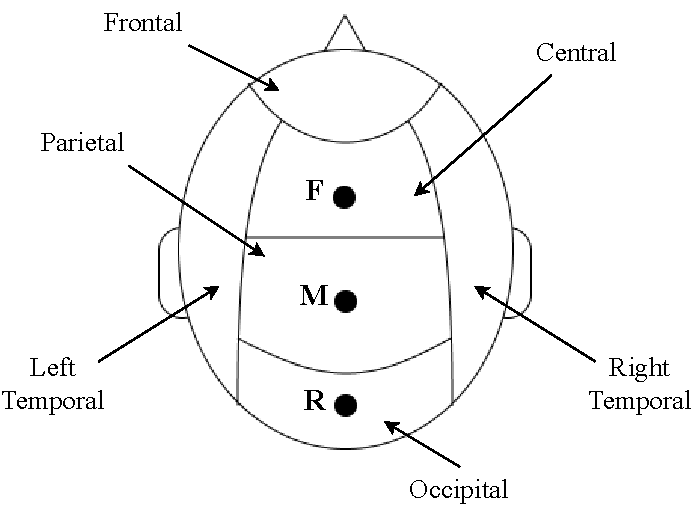
\includegraphics[width=0.42\textwidth]{images/tactor-placement.pdf}
    \caption{Diagram shows placement of actuators in different regions of the head. The front actuator (F) lies in the central region, middle (M) in the parietal, and rear (R) in the occipital.}
    \label{fig:head-regions}
\end{figure}



\subsection{Vibrotactile Distance Encodings}
To understand how the following distance can be converted into a vibrotactile signal, we consider the previously identified encoding parameters: the location, rhythm, duration, frequency, amplitude, and waveform of a vibrotactile stimuli \cite{guidelines, 10.5555/976310.976313}. The parameters of frequency and amplitude, which typically have 5-7 perceptually distinguishable levels \cite{guidelines}, are encompassed within the candidate parameter \textit{'intensity'}. However, in our context of use, where the stimuli recipient receives haptic interference from the terrain they cycle over, the number of distinguishable levels reduce, making a 3-level distance category unsuitable. Additionally, the waveform of our stimuli signal is restricted by our actuators, which are only capable of producing sine waves.

This leaves the parameters of location, rhythm, and duration to be used to encode distance. Prior work has typically used location to convey direction. However, in our system, we do not convey the specific direction of the vehicle; instead, we only prompt the rider to look behind, meaning this parameter is left free.

Rhythm is a complex parameter where a number of stimuli are delivered in succession to compose a pattern. Similarly, duration can refer to multiple different attributes, such as the length of a stimulus, or overall length of a cue. How the terms \textit{rhythm} and \textit{duration} are defined is unclear and changes across many previous works. McDaniel et al. \cite{10.1145/1520340.1520718} used rhythm by varying the \textit{delay} between two 50ms stimuli in a cue. Pielot et al. \cite{10.1145/1753326.1753581} used rhythm by varying the \textit{number} of 200ms stimuli with a 200ms delay between each, and referred to duration as the \textit{length} of a single stimulus. Asif et al. \cite{10.1145/1868914.1868923} also used rhythm by varying the \textit{number} of stimuli in a cue; however, as the number of stimuli increases, their \textit{duration} and \textit{delay} between each decreased, keeping the \textit{overall duration} of the rhythm constant. Their combined rhythm and duration encoding similarly kept the \textit{overall duration} of the rhythm constant, but instead also kept the \textit{duration} and \textit{delay} of the varying number of stimuli constant.

In the following study, we explicitly define \textit{duration} and the exact parameters which compose the term \textit{rhythm}, and investigate how these parameters can be used alongside \textit{location} to encode distance.



\section{Lab Study - Investigating Vibrotactile Distance Encodings}\label{sec:lab-study}
The goal of this experiment was to investigate how different distance categories could be effectively encoded and conveyed, using vibrotactile cues delivered from a cycling helmet. We compared six defined encoding schemes which were composed of different \textit{patterns} and \textit{durations}. The evaluation investigated the following sub-questions from our first primary research question:
\begin{enumerate}[label=RQ1.\arabic*.]
    \item Is the sagittal plane of the scalp a suitable location for vibrotactile stimulation?
    \item Which combinations of pattern and duration encodings are most usable?
    \item Which combinations of pattern and duration encodings gives the lowest number of information perception/interpretation errors?
\end{enumerate}


\subsection{Experiment Design}
\subsubsection{Independent Variables}
The experiment centered around the delivery of distance information, which was composed of three independent variables: the distance category, the vibration pattern, and cue duration. The combination of the pattern and duration created six unique experimental conditions, known as the distance encoding schemes. When combined with the three distance categories (\textit{far}, \textit{near}, and \textit{imminent}), they create 18 vibrotactile cues. How the pattern and duration effect the parameters of a vibrotactile cue can be seen in Table \ref{tab:location} and Figure \ref{fig:cue-table}.

\textbf{Pattern:} The vibration pattern is a composite parameter, which combines the location of a vibration (the activated actuator), and the delay between delivered stimuli (also known as the inter-stimulus-interval). The vibration pattern had three distinct levels: \textit{Singular}, \textit{Wall}, and \textit{Wave}. With a \textit{Singular} pattern, only a single actuator at the location relative to the specified distance is activated. With a \textit{Wall} pattern, all actuators, from the rear to the one at the location relative to the specified distance, are activated simultaneously. The \textit{Wave} pattern works similarly, however, there is a delay of 150ms between each actuators activation. These pattern names are inspired from a pilot study with a single participant, who described the feeling of the patterns as \textit{‘creating a wall’} or \textit{‘moving like a wave across your head’}. 

\textbf{Duration:} In this study, we define duration as the number of times a vibrotactile cue is delivered and had two distinct levels: \textit{Constant} and \textit{Varying}. With a \textit{Constant} duration, each vibration cue was delivered only once. With a \textit{Varying} duration, the number of times a cue is delivered increased as the distance decreased. 


\begin{table*}[h]
    \centering
    \begin{tabular}{l||c|c|c||c|c}
        & \multicolumn{3}{c||}{PATTERN (Location + ISI)} & \multicolumn{2}{c}{RHYTHM DURATION}\\ \cline{2-6} 
        \emph{Distance Cue} & \emph{Singular (ISI=0)} & \emph{Wall (ISI=0)} & \emph{Wave (ISI=150ms)} & \emph{Constant} & \emph{Varying} \\ \hline
        Far & R & R & R & 1 & 1\\ 
        Near & M & R+M & R$\rightarrow$M & 1 & 2\\ 
        Imminent & F & R+M+F & R$\rightarrow$M$\rightarrow$F & 1 & 3\\ 
    \end{tabular}
    \caption{Table shows the activated actuators and number of deliveries for each distance, pattern and duration level. R, M, and F refers to the Rear, Mid, and Front actuator respectively. + denotes simultaneous activation and $\rightarrow$ denotes delayed activation.}
    \label{tab:location}
\end{table*}

\begin{figure*}[h]
    \centering
    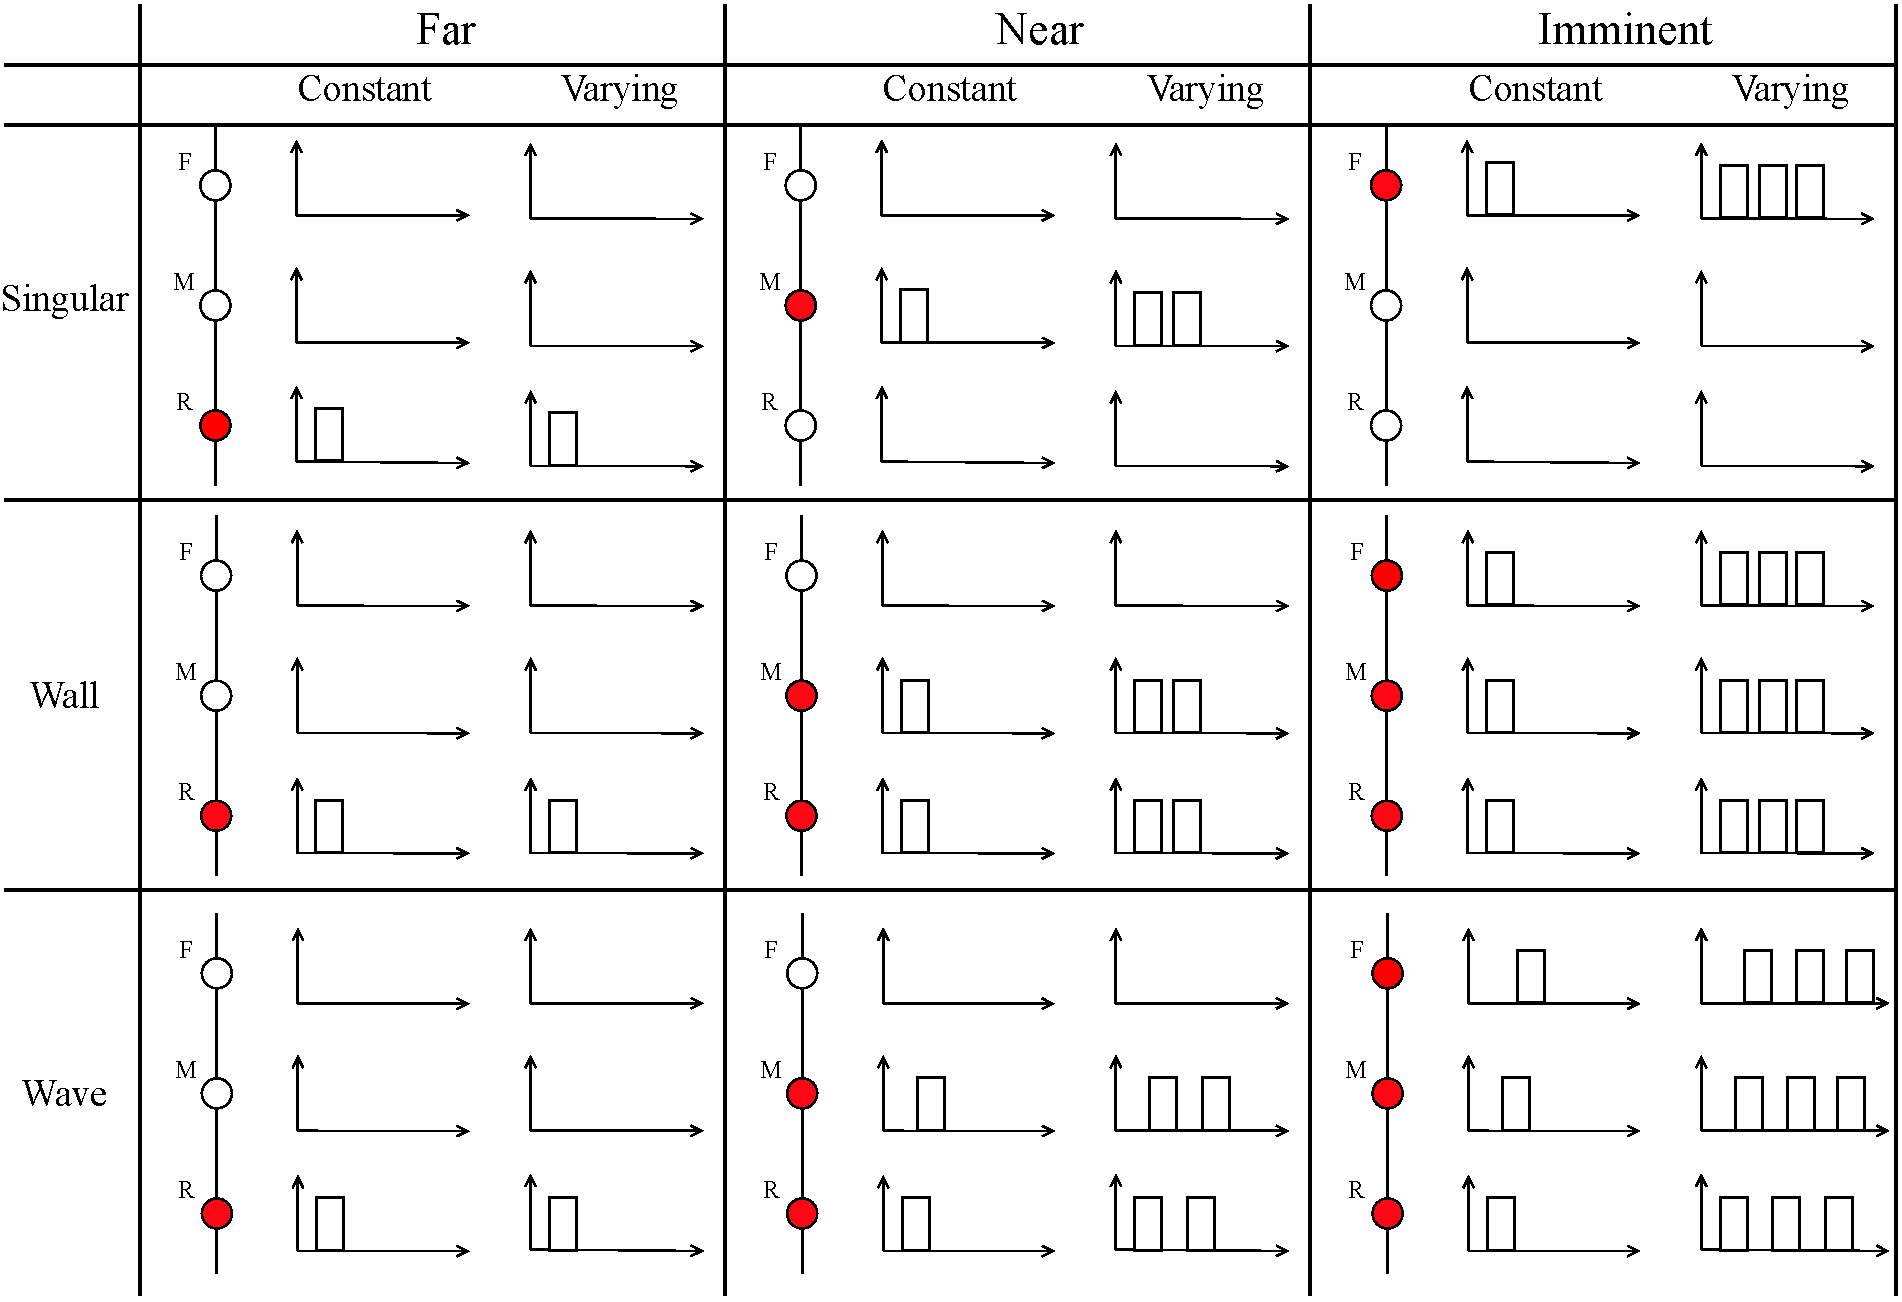
\includegraphics[width=0.75\textwidth]{images/cue-table.pdf}
    \caption{Diagram shows the vibrotactile cues delivered to each actuator, depending on the distance, pattern, and duration.}
    \label{fig:cue-table}
\end{figure*}



\subsubsection{Apparatus and Encoding Parameters}\label{sec:apparatus}
The helmet with the described configuration of tactile actuators was used to deliver the vibrotactile cues. In this paper, we define a vibrotactile cue to be the composition of a number of tactile rhythms, and define a rhythm to be the composition of a number of tactile stimuli.

\textbf{Stimuli Parameters:} We define a stimulus to have four possible parameters: (i) intensity (frequency + amplitude), (ii) waveform, (iii) location, and (iv) stimulus duration. Each actuator produced sinewaves and was set to vibrate at its maximum intensity, with a duration of 300ms. The possible locations were one of three actuators: the \textit{front}, \textit{middle}, and \textit{rear}, and was dependent upon the encoding scheme.

\textbf{Rhythm Parameters:} We define a rhythm to have three possible parameters: (i) inter-stimulus-interval (ISI), (ii) number of stimuli deliveries, and (iii) length of the rhythm. Often referred to as the 'delay', the ISI is the time between consecutive stimuli in a rhythm, and when combined with the location, became our \textit{pattern} variable. The number of stimuli deliveries is the number of times that a single actuator is activated per rhythm, and was set to a constant value of 1. The overall length of the rhythm is dependent upon these prior parameters.

\textbf{Cue Parameters:} We define a cue to have three possible parameters: (i) inter-rhythm-delay, (ii) number of rhythm deliveries, and (iii) length of the cue. The inter-rhythm-interval is the time between consecutive rhythms, and was set to a constant 100ms. The number of times that a rhythm is delivered per cue was our \textit{duration} variable, and was dependent on the encoding scheme. The overall length of the cue is dependent upon these prior parameters.


\subsubsection{Participants}
20 participants were recruited for the study, all aged 16-24 years old. However, the helmet did not fit P13, therefore they could not participate in the study.


\subsubsection{Dependent Measures}
Following our defined research questions for the evaluation, we determine our dependent measures to be the usability of the encoding schemes, and the information perception of participants using such schemes. We measure the usability of an encoding scheme in terms of its usefulness, distinguishability, interpretability, intuitiveness, and length of its cues. This is measured using a combination of qualitative feedback and 5-point Likert scale questions in a post-experiment questionnaire \cite{joshi2015likert}. We measure information perception by recording the errors made by participants in identifying the correct cues. Finally, we analyse participants responses to the applied questionnaire to further understand additional related factors, such as their perception of the actuators, the comfort of the helmet, and their understanding of following distance.

\begin{table*}[h]
    \centering
    \begin{tabular}{l|c|c|c|c|c}
        \emph{Encoding Scheme} & \emph{Useful.} & \emph{Distin.} & \emph{Interp.} & \emph{Intuit.} & \emph{Length} \\ \hline
        Singular Constant & 3.05 ± 1.31 & 2.79 ± 1.13 & 2.95 ± 1.03 & 3.79 ± 0.92 & 3.00 ± 1.15 \\ 
        Singular Varying & 4.42 ± 0.77 & 4.26 ± 0.93 & 4.42 ± 0.61 & 4.53 ± 0.61 & 3.89 ± 1.05 \\ 
        Wall Constant & 2.74 ± 1.19 & 1.95 ± 1.03 & 2.42 ± 1.07 & 3.42 ± 1.12 & 3.11 ± 1.15 \\ 
        Wall Varying & 4.32 ± 0.88 & \textbf{4.42 ± 0.84} & 4.47 ± 0.70 & 4.58 ± 0.51 & \textbf{3.89 ± 1.33} \\
        Wave Constant & 3.58 ± 1.02 & 2.84 ± 1.12 & 3.47 ± 1.17 & 4.16 ± 0.83 & 3.58 ± 1.12 \\
        Wave Varying & \textbf{4.58 ± 0.51} & 4.37 ± 0.90 & \textbf{4.53 ± 0.70} & \textbf{4.63 ± 0.76} & 3.74 ± 1.20 \\
    \end{tabular}
    \caption{Table shows the mean and standard deviation of the Likert scores for each encoding scheme for each measure of usability. Likert scores are measured on a five-point scale (1 - Strongly Disagree, 5 - Strongly Agree). The highest score in each category is emboldened.}
    \label{tab:usability-scores}
\end{table*}

\subsubsection{Procedure}
Each experimental session began by first briefing the participant on the study’s purpose and explaining how the TactiHelm system operates. Participants were allowed to wear the helmet and adjust the tightness until they were comfortable with its placement. They were presented a diagram which showed the positioning of the actuators inside the helmet (Figure \ref{fig:head-regions}) and the evaluator activated each one, repeating any if a participant requested. The evaluator gave a brief explanation of the term \textit{“following distance”}, and explained the three categories we have divided this value into. Participants were then asked to complete the first part of the provided questionnaire, regarding their initial thoughts towards the aforementioned described concepts.

To compare the six encoding schemes, we used a within-subjects design, where each participant evaluated every scheme under lab conditions. This process was split based on the three levels of vibration pattern. Participants were sequentially introduced to each pattern level, under which they evaluated both duration levels and completed part of the provided questionnaire, before advancing to the next subsequent pattern level. This approach enabled participants to provide feedback on the two most recent encoding schemes immediately after evaluation, ensuring that their impressions were accurately captured. The evaluation order of the schemes was balanced using a Latin square.

The evaluation of a scheme was composed of three trials. During a trial, a vibrotactile cue representing a distance would be sent to the helmet every five seconds. Participants would then have to state which distance they believed was just conveyed. The first trial was a short training phase, aimed to quickly train participants on how to interpret the encoding scheme. The second and third trials were part of the data gathering phase, where participants' results would be recorded without correction. This totalled to 18 trials for each participant. Trials were consistent in length: every training trial had a total of seven cues, whereas every data gathering trial had 12 cues, with an equal split of different distances. The order of the trials remained constant.


\subsection{Results}
The following presents the acquired results from our study. Friedman's ANOVA tests were applied to Likert data from the questionnaire, followed by Wilcoxon tests on each pair of conditions. For the cue perception errors, we applied a two-way repeated measures ANOVA, to compare the means of the number of correct guesses across the six schemes and three distance cues. This was followed by pairwise t-tests across these two groups. For the Wilcoxon tests, a Bonferroni correction was applied to the standard alpha value of 0.05, to account for the number of comparisons (\textit{N}=3) in each group \cite{Armstrong2014-vr}. The means and standard deviations for each usability measure can be seen in Table \ref{tab:usability-scores}. Tables \ref{tab:usability-stats} and \ref{tab:cue-perception-stats} show the results of the post-hoc Wilcoxon and t-tests.



\subsubsection{Usability of Encoding Schemes}
The applied Friedman tests showed that there were significant differences across all our measures of usability: usefulness (\textit{Chi-Square}=49.16, \textit{p}<.05), distinguishability (\textit{Chi-Square}=58.04, \textit{p}<.05), interpretability (\textit{Chi-Square}=51.37, \textit{p}<.05), intuitiveness (\textit{Chi-Square}=32.82, \textit{p}<.05), and length of cues (\textit{Chi-Square}=14.09, \textit{p}<.05).

\textbf{\textit{Constant} vs \textit{Varying} durations within each pattern:} The Wilcoxon tests revealed that within each pattern category, there were significant differences between the two duration conditions, with the \textit{Constant} conditions repeatedly outperforming the \textit{Varying} conditions across all usability measures.

\textbf{\textit{Single} vs \textit{Wall} vs \textit{Wave} patterns within the \textit{Constant} duration:} The Wilcoxon tests revealed that when comparing the \textit{Single} and \textit{Wall} patterns with a \textit{Constant} duration, the only significant differences was between their distinguishability, where the \textit{Single} condition was ranked better. In-fact, the \textit{Wall Constant} scheme was ranked the worst across all the usability measures, with the exception of the length of the cue, where participants ranked the \textit{Single Constant} scheme the lowest. Comparing the \textit{Wave} condition to the other two, we see that significant differences were found in many of the usability measures, with the \textit{Wave Constant} scheme being ranked the highest or near highest by participants across all dimensions.

\textbf{\textit{Single} vs \textit{Wall} vs \textit{Wave} patterns within the \textit{Varying} duration:} When comparing the different pattern conditions for a \textit{Varying} duration, there were no significant differences found across any usability measure, with all the \textit{Varying} schemes being rated equally high.


\begin{table*}[h]
    \centering
    \begin{tabular}{l|ccccc}
        \toprule
        Comparison & \emph{Useful.} & \emph{Distin.} & \emph{Interp.} & \emph{Intuit.} & \emph{Length}\\ \midrule
        Sing-Con. vs Sing-Var. & \textbf{W=0.0, p<.001} & \textbf{W=0.0, p<.001} & \textbf{W=0.0, p<.001} & \textbf{W=4.0, p=.008} & \textbf{W=7.0, p=.011} \\
        Wall-Con. vs Wall-Var. & \textbf{W=15.5, p=.002} & \textbf{W=0.0, p<.001} & \textbf{W=3.0, p<.001} & \textbf{W=0.0, p<.001} & W=15.0, p=.056 \\
        Wave-Con. vs Wave-Var. & \textbf{W=5.5, p=.001} & \textbf{W=0.0, p<.001} & \textbf{W=14.5, p=.008} & W=11.0, p=.041 & W=33.5, p=.659 \\ \midrule
        Sing-Con. vs Wall-Con. & W=32.5, p=.35 & \textbf{W=8.5, p=.028} & W=25.0, p=.145 & W=13.5, p=.131 & W=23.0, p=.627 \\
        Sing-Con. vs Wave-Con. & \textbf{W=3.0, p=.031} & W=68.0, p=1.00 & W=36.0, p=.166 & W=9.0, p=.100 & W=9.0, p=.055 \\
        Wall-Con. vs Wave-Con. & \textbf{W=2.5, p=.010} & \textbf{W=10.0, p=.006} & \textbf{W=5.5, p=.001} & \textbf{W=5.0, p=.005} & W=10.5, p=.075 \\ \midrule
        Sing-Var. vs Wall-Var. & W=19.0, p=.668 & W=21.0, p=.49 & W=30.0, p=.763 & W=6.0, p=.655 & W=22.5, p=1.00 \\
        Sing-Var. vs Wave-Var. & W=2.0, p=.257 & W=16.0, p=.773 & W=10.5, p=.527 & W=3.5, p=.577 & W=12.0, p=.366 \\
        Wall-Var. vs Wave-Var. & W=12.0, p=.19 & W=25.5, p=.834 & W=43.0, p=.851 & W=10.5, p=.527 & W=12.0, p=.366 \\
        \bottomrule
    \end{tabular}
    \caption{Table shows the Wilcoxon tests results for each usability measure, found between different conditions. A Bonferroni corrected alpha value of 0.017 was used. Significant values are emboldened.}
    \label{tab:usability-stats}
\end{table*}


\begin{table*}[h]
    \centering
    \begin{tabular}{l|c|c|c}
        \toprule
        Comparison & \emph{Far} & \emph{Near} & \emph{Imminent} \\ \midrule
        Sing-Con. vs Sing-Var. & t=-0.64, p=.531 & t=-1.37, p=.187 & \textbf{t=-3.39, p=.003} \\
        Wall-Con. vs Wall-Var. & t=-1.92, p=.070 & \textbf{t=-3.01, p=.007} & \textbf{t=-5.41, p<.001} \\
        Wave-Con. vs Wave-Var. & t=-0.85, p=.408 & \textbf{t=-2.36, p=.030} & \textbf{t=-2.62, p=.017} \\ \midrule
        Sing-Con. vs Wall-Con. & t=0.00, p=1.00 & t=1.78, p=.092 & \textbf{t=2.87, p=.010} \\
        Sing-Con. vs Wave-Con. & t=-0.14, p=.891 & t=0.56, p=.586 & t=0.29, p=.776 \\
        Wall-Con. vs Wave-Con. & t=-0.17, p=.867 & t=-1.29, p=.213 & \textbf{t=-4.02, p<.001} \\ \midrule
        Sing-Var. vs Wall-Var. & t=-1.23, p=.235 & t=-0.29, p=.772 & t=0.52, p=.607 \\
        Sing-Var. vs Wave-Var. & t=-0.27, p=.790 & t=-0.62, p=.542 & t=0.00, p=1.00 \\
        Wall-Var. vs Wave-Var. & \textbf{t=2.19, p=.042} & t=-0.57, p=.578 & t=-0.81, p=.429 \\
        \bottomrule
    \end{tabular}
    \caption{Table shows the t-tests results for the perception of distance cue, found between different conditions. An alpha value of 0.05 was used. Significant values are emboldened.}
    \label{tab:cue-perception-stats}
\end{table*}



\subsubsection{Information Perception}
Information perception was measured by recording the number of errors made by participants in identifying the correct distance cues. Figure \ref{fig:mean-correct} presents these results for each distance category for each scheme. Our two-way ANOVA test revealed there were statistically significant differences between pairs of schemes (\textit{F}=9.25, \textit{p}<.05) and distance cues (\textit{F}=14.86, \textit{p}<.05), and there was a significant interaction between these two groups (\textit{F}=6.83, \textit{p}<.05).

\textbf{Differences in cue perception within schemes:} The t-tests revealed there was a significant difference in cue perception between the \textit{far} (\textit{M}=96.16\%, \textit{SD}=4.70\%) and \textit{imminent} (\textit{M}=87.94\%, \textit{SD}=8.98\%) distance cues; \textit{t}=4.54, \textit{p}<.05. However, the only scheme to exhibit this difference was the \textit{Wall Constant} scheme; \textit{t}=5.25, \textit{p}<.05. Similarly a significant difference was found between the \textit{imminent} and \textit{near} (\textit{M}=94.30\%, \textit{SD}=5.23\%) cues; \textit{t}=-3.78, \textit{p}<.05. However, this was only seen in the \textit{Singular Constant} (\textit{t}=-2.69, \textit{p}<.05) and \textit{Wall Constant} (\textit{t}=-3.36, \textit{p}<.05) schemes. There was no significant difference found between the \textit{far} and \textit{near} cues; \textit{t}=1.58, \textit{p}=0.13.

\textbf{Far Cue:} The only statistically significant difference found via the t-tests for the far distance cue, was between the \textit{Wall} and \textit{Wave Varying} scheme; \textit{t}=2.19, \textit{p}<.05.

\textbf{Near Cue:} Significant differences for the near distance cue were revealed between the Wall Constant and Varying schemes (\textit{t}=-3.01, \textit{p}<.05), and the Wave Constant and Varying schemes (\textit{t}=-2.36, \textit{p}<.05). 

\textbf{Imminent Cue:} Significant differences for the imminent cue were found between the \textit{Constant} and \textit{Varying} durations for each pattern: \textit{Singular} (\textit{t}=-3.39, \textit{p}<.05), \textit{Wall} (\textit{t}=-5.41, \textit{p}<.05), and \textit{Wave} (\textit{t}=-2.62, \textit{p}<.05). Additionally, significant differences were found between schemes with a \textit{Constant} duration, namely the \textit{Singular} and \textit{Wall} (\textit{t}=2.87, \textit{p}<.05), and \textit{Wall} and \textit{Wave} (\textit{t}=-4.02, \textit{p}<.05) conditions.

\textbf{Recognition errors across schemes:} Figure \ref{fig:heatmaps} shows the ratio of recognised distance cues guessed by participants, for each cue, for each scheme. Far cues were rarely misinterpreted; however, when they were, they were typically misinterpreted as near cues. Near cues were also typically correctly recognised, with the exception of within the \textit{Wall Constant} scheme, where 14.47\% were misinterpreted as imminent cues. Imminent cues were highly recognised across the \textit{Varying} schemes; however, these were typically misinterpreted as a near cue in the \textit{Constant} schemes, such as in the \textit{Wall Constant} scheme where 32.89\% were misinterpreted as near. Imminent cues were also the most commonly missed, with 3.29\% missed with the \textit{Singular Constant} scheme. 



\begin{figure}[h]
    \centering
    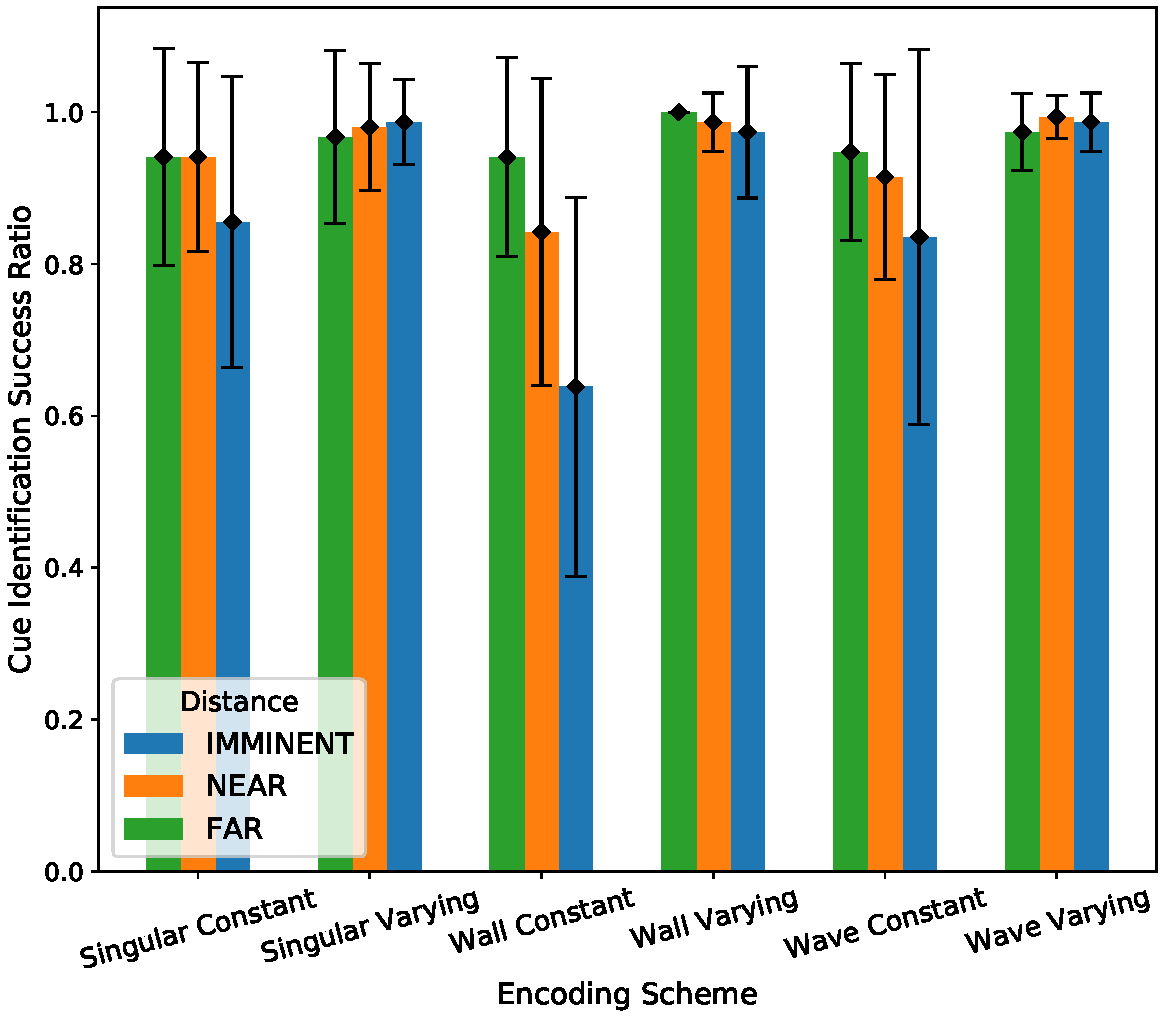
\includegraphics[width=0.44\textwidth]{dissertation/images/Mean Correct by Encoding Scheme.pdf}
    \caption{Cue identification success ratio of each distance cue across the six schemes.}
    \label{fig:mean-correct}
\end{figure}

\begin{figure}[h]
    \centering
    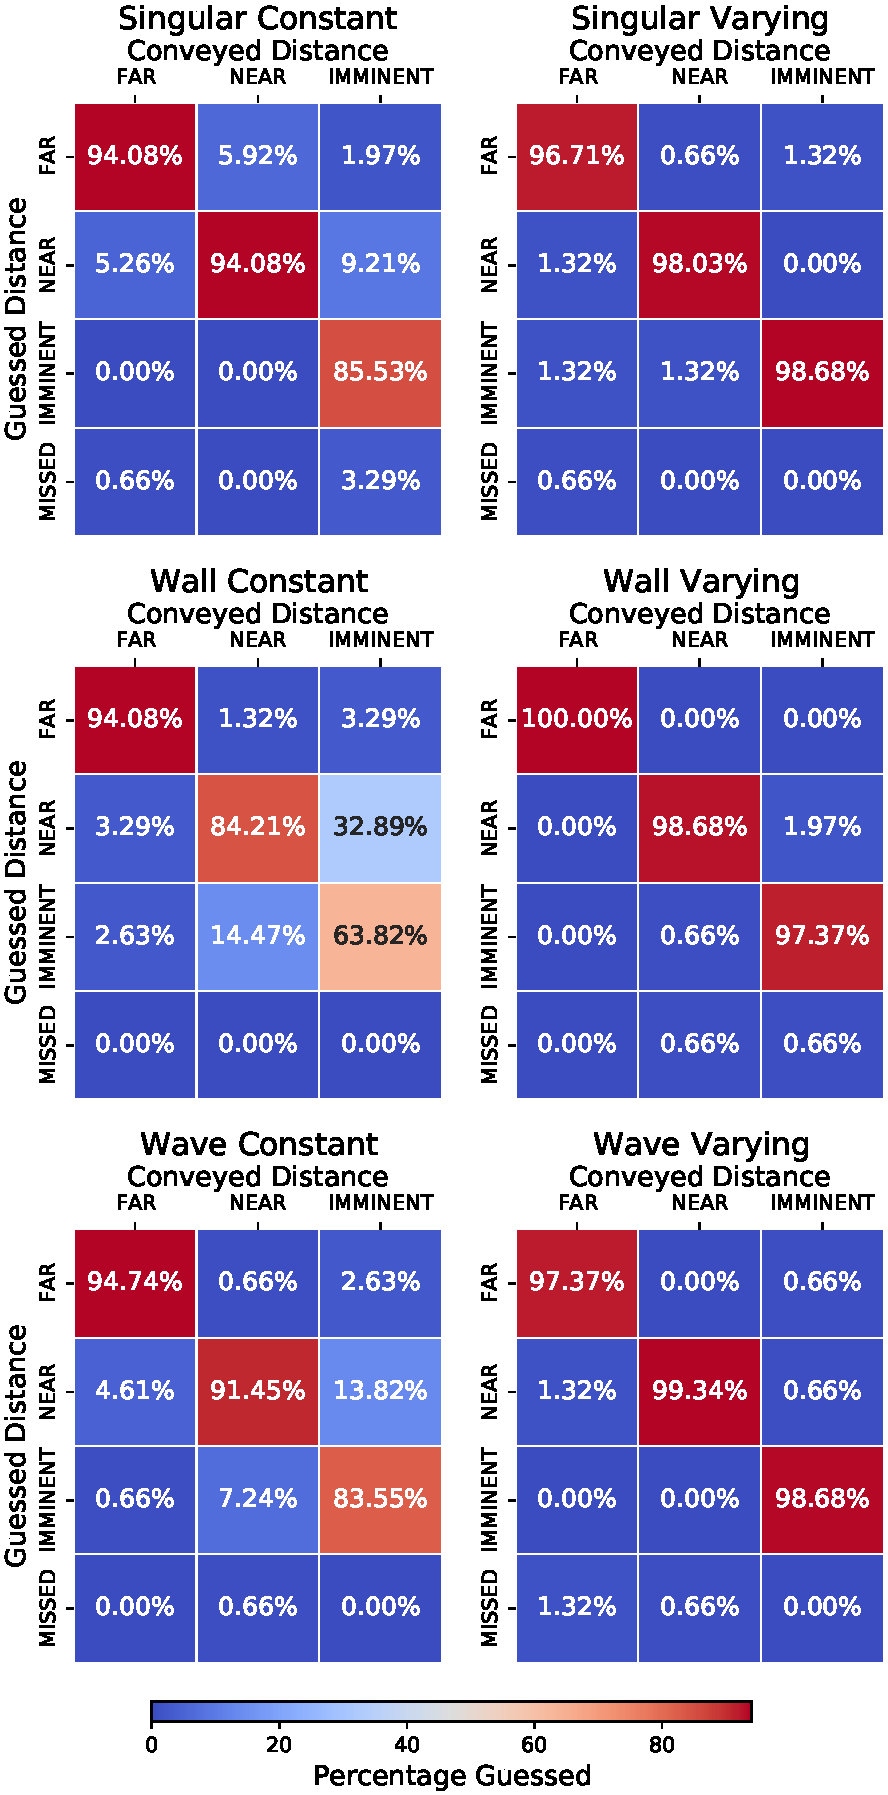
\includegraphics[width=0.40\textwidth]{dissertation/images/heatmaps.pdf}
    \caption{Percentage of guessed distance cues for each distance per scheme.}
    \label{fig:heatmaps}
\end{figure}




\subsubsection{Further Comments and Observations}
\textbf{Scheme Preference:}
Participants ranked the six schemes in order of preference. A Friedman's test revealed there were significant differences in their rankings (\textit{Chi-Square}=47.90, \textit{p}<.05). All of the \textit{Varying} conditions were ranked higher than their \textit{Constant} counterparts, with the \textit{Wave} condition being the highest ranked, followed by the \textit{Wall} then \textit{Singular} condition. The Wilcoxon tests revealed significant differences between every combination of these schemes.

\textbf{Perception of the Actuators:} Participants were asked to rate the perception of the three tactile actuators using a 5-point Likert scale. Applying the Friedman's test revealed that there were no statistically significant differences between the perception of the Front (\textit{M}=3.42, \textit{SD}=1.35), Middle (\textit{M}=3.84, \textit{SD}=1.12), and Rear (\textit{M}=4.11, \textit{SD}=1.20) actuators; \textit{Chi-Square}=3.76, \textit{p}=.15. However, participants often stated that the front and middle actuators were harder to perceive: \textit{"I was able to distinguish location on my head. However the middle and front tactors were much harder to feel than the back one"} [P3].

\textbf{Layout of the Actuators:} Following our initial explanation and survey questions, 85\% of participants correctly answered that the actuator at the back of the head would be activated if a detected vehicle was \textit{far}. Additionally, participants stated that they agreed with the configuration of the actuators, \textit{"The layout made sense in relation to the problem and the tactors are sufficiently powerful"} [P7]. However, multiple participants stated that the actuators often felt too close to each other, expecting the front one to be closer to the forehead, \textit{"I expected the middle one to be where the front is and the front one to be more towards the forehead"} [P11].

\textbf{Helmet Comfort:}
Regarding the comfort of the helmet, participants gave an average rating of 7.15 out of 10 for its' comfortableness (\textit{SD}=2.08), with many commenting that its weight and small size caused uncomfortable pressure points, such as at the back of the head. 

\textbf{Understanding of Following Distance}
From our initial explanation of the following distance, few participants (25\%) correctly understood that it was in-fact a measure of time and hence typically measured in seconds. From this group, a variety of answers were provided, regarding what value the distance would be, given a vehicle was \textit{imminent}, ranging from one to five seconds. Of the 75\% of participants who did not correctly understand, their answers were typically measured using either metres or car/bike lengths. These ranged from one to five metres or one to two car/bike lengths. These answers did not mention what speed the vehicle would be travelling at. However, the majority of participants were not avid cyclists, with only 30\% stating they cycle more than one hour per week, meaning their interpretation of this term may differ from our target group. When asked whether or not they believed the following distance would be an appropriate indicator of an approaching vehicle, most participants agreed that it would be, and agreed with the categorisation of this metric into three values.




\subsection{Discussion}
The aim of this study was to explore how the pattern and duration of a vibrotactile rhythm on the head could be used to effectively encode distance. By gathering qualitative feedback regarding usability measures and recording participants information perception errors across different encoding schemes and cues, we answer our previously defined research questions.

\textbf{RQ1.1 (suitability of the head as a vibrotactile display):} The configuration of the tactile actuators in our helmet was well received, with the majority of participants correctly understanding, how the layout of the actuators relate to the distance of an approaching vehicle. However, multiple participants stated they felt that the front and middle actuators were too close together, and that the front one could have been shifted closer towards the forehead to aid localisation and make the stimuli more distinguishable. This was likely related to their lower perception ratings, compared to the rear actuator. However, there are multiple further reasons which can explain the difficulty in perception. For example, as previously discussed, the front of the scalp is less perceptible than the back \cite{headguidelines, MYLES2015177, 7463147}. Additionally, variance in head size meant that some participants' scalp pressed less against the top of the helmet than others, leading to a lesser perceived intensity. Because of the difficulty in perception, multiple participants stated they relied on the sound of the vibration rather than the tactile feeling. An improved experimental design would have had participants wear noise cancelling headphones to block this sensory channel; we acknowledge this as a limitation in our study.

\textbf{RQ1.2 \& RQ1.3 (most effective encoding scheme):} In terms of both usability and cue perception, all \textit{Varying} conditions performed better than all \textit{Constant} conditions. This was likely due to the ability of being able to easily count the number of vibrations, opposed to the comparably harder task of having to identify the position of the stimuli on the head, as expressed by the majority of participants. This suggests that encoding distance using the duration of a rhythm (specifically the number of cue deliveries) does not inherently make it more effective, but rather it creates an easily perceptible counting mechanism, from which inferring the distance is less cognitively demanding, and thus easier. Such inferences are harder to make when relying upon the location of a stimuli, which requires more cognitive demand to translate to a distance. For example, it is less cognitively demanding to infer an imminent distance from counting three buzzes, that it is by having to identify the precise location of the vibration. 

This dominant effect of varying the duration can be seen in the lack of significant differences within the \textit{Varying} schemes, suggesting the pattern, and hence location, is insignificant in comparison. However, despite few significant differences in cue perception, participants rated the \textit{Wave} condition best of all \textit{Constant} schemes, in terms of usability and preference. This could be because of the saltation sensory illusion it creates, which simulates the feeling of movement across the active stimulus loci \cite{cholewiak2000generation, geldard1975sensory, peeters2019vibrotactile}, thus better representing the feeling of an approaching vehicle. The low cue perception of the \textit{Wall Constant} scheme can be similarly explained by the funneling illusion, where the perceived location of a tactile stimulus is in-between two or more stimulus loci \cite{gardner1972sensory, 5710913, s150407913}, causing participants to misinterpret the cues. Whether improving localisation of the stimuli would have an affect on the ease of perception is left to suggested future work.

\textbf{Conclusion:} From this study, it is evident that our configuration of actuators along the sagittal plane of the scalp, is suitable for conveying the concept of an approaching vehicle. Although, we may aid distinguishability of these tactors be increasing the spacing between the front and middle actuators. We find that the location of vibrotactile rhythm on the scalp is insignificant in comparison to its duration and perceived intensity, as shown by participants preference to \textit{Varying} schemes. However, when comparing the rhythmic patterns which vary the location and delay between delivered stimuli, participants preferred the \textit{Wave} scheme, which created a sensation of movement across the scalp. Therefore in our following study, we aim to assess the effectiveness of using our defined \textit{Wave Varying} encoding scheme to encode our three levels of distance.


\section{User Study - TactiHelm Evaluation}\label{sec:user-study}
The goal of this experiment was to evaluate our developed TactiHelm system in the real world. Specifically, we assessed its usability and effectiveness in warning users of the presence and proximity of approaching vehicles behind them, all within a naturalistic setting. Through this study, we aimed to answer the following questions:
\begin{enumerate}[label=RQ2.\arabic*.]
    \item Can participants accurately perceive and interpret our defined vibrotactile cues on the scalp whilst cycling?
    \item Does the use of TactiHelm improve participants' perceived safety and comfort whilst cycling with other road vehicles?
    \item Is our 3-level categorisation of following distance into far, near, and imminent, appropriate for our proposed safety system?
\end{enumerate}

\subsection{Experiment Design}
Commuter cyclists were recruited and equipped with a bike radar, the TactiHelm helmet, and a microphone to record their home to office commute. We asked participants to use TactiHelm on their normal commuting routes and to perform a think-aloud evaluation - audibly expressing any thoughts and feelings regarding the effectiveness of the helmet at warning them of approaching vehicles. Outwith of this, we asked them to behave as they normally would.

After completing their commutes, participants were asked to complete a post-evaluation questionnaire, followed by a brief, semi-structured interview with the evaluator. The questionnaire included questions from the NASA-RTLX \cite{doi:10.1177/154193120605000909} and the System Usability Scale \cite{sus} questionnaire. Following this, participants were asked to perform an additional commute, without using TactiHelm, after which they would complete the NASA-RTLX questionnaire again. This was to establish a baseline score for comparison. We analysed participants' captured audio for any qualitative comments made during the evaluation. 

\subsubsection{Dependent Measures}
We used three primary dependent measures to evaluate the effectiveness of our system: 1) NASA-RTLX data to measure participants workload whilst cycling, both with and without TactiHelm, 2) SUS data to measure the usability of TactiHelm, and 3) qualitative comments made during the think-aloud evaluation, questionnaire, and interview. We primarily looked for comments regarding the accuracy and effectiveness of the vibrotactile warnings, and the perceived safety and awareness of the participant. We also noted comments related to additional factors of the helmet, such as its comfort. Friedmans' ANOVA tests were applied to 5-point Likert-style questions from the questionnaire, and paired t-tests were applied to the NASA-RTLX data.

\subsubsection{Participants}
Five commuter cyclists were recruited for the study, (\textit{16-24 years}=5, \textit{55-64 years}=1). An additional participant was also recruited, however, the TactiHelm system did not work on their commutes; therefore, they were unable to provide any meaningful data. All participants were affiliated with the university to allow ease of communication due to the requirement of handling the equipment.

\subsubsection{Apparatus}
The full TactiHelm system was used for this study, as seen in Figure \ref{fig:setup}. Following analysis of the results from the previous study, the \textit{Wave Varying} encoding scheme was used to encode the following distance of approaching vehicles. Preliminary testing was carried out by the researchers, to find the ideal threshold values at which to define the distance categories (as seen in Table \ref{tab:fd-thresholds}). Whether or not these values are optimal, we seek to answer in this study.

The TactiHelm helmet was improved to have a more light-weight and robust design. The vents of the helmet were utilised to hold a smaller sized breadboard and the front actuator was moved closed to the front of the head to increase the space from the middle actuator. A rain-cover was also added, which would: a) protect the electronic components from rain, b) keep the components contained within the helmet, and c) improve the helmet's perceived social acceptability among participants, by concealing the components, helping minimise any social discomfort.

As the controller application was compatible exclusively with Android devices, participants were provided with such a device, for the duration of the study, with the required applications already downloaded. Participants were additionally provided with a microphone to record the think-aloud, the Garmin Varia RTL515 bike radar, and a bike phone-holder, to hold the mobile device.

\vspace{.15cm}
\begin{table}[h]
    \centering
    \begin{tabular}{l|c}
        \emph{Distance Cue} & \emph{Following Distance (ms)} \\ \hline
        Far & $\geq$3500 \\ 
        Near & >1500 and <3500 \\ 
        Imminent & $\leq$1500  \\ 
    \end{tabular}
    \caption{Table shows the following distance thresholds which define the three distance cues.}
    \label{tab:fd-thresholds}
\end{table}


\subsubsection{Procedure}
Participants attended a briefing session where we explained the study's purpose and how to use the provided equipment and associated software. We demonstrated how to turn on and off the helmet and bike radar, and how to use the TactiHelm Controller application to connect to them and to start receiving vibrations. We instructed participants to record their route using the 'Ride with GPS' mobile application. If a participant stated they were not comfortable sharing their GPS data, they were instead asked to provide general information of their commute, such as its estimated distance and time to complete. Participants were also briefed on how to use the microphone and how to perform a think-aloud evaluation. We encouraged them to regularly articulate their thoughts out-loud and provided guidance on what to say, prompting them to describe what they see and feel. However, we instructed them not to concentrate too hard on the evaluation so as to not distract them, and to behave as they normally would. Participants were given the helmet to wear as we demonstrated the three possible cues they may feel. Additionally, they were provided with a user manual in case they forgot how to use the equipment and software. 

Participants were then tasked with recording two commutes - from their work to their residence and vice versa. They were trusted to keep the equipment overnight and return it the following day. Immediately following their second commute, they were prompted to complete the post-experiment questionnaire. Participants were then instructed to repeat their second commute, from their residence to their workplace, without the aid of TactiHelm. Following this, they were to complete the NASA-RTLX part of the questionnaire once more. A period of seven days was allotted for this task. Upon completion, they were fully debriefed. The study was approved by the University’s ethics committee.

\begin{table*}[h]
    \centering
    \begin{tabular}{l|ccccc|ccccc|cc}
    \multicolumn{1}{c|}{} & \multicolumn{5}{c|}{WITH TACTIHELM} & \multicolumn{5}{c|}{WITHOUT TACTIHELM} & \multicolumn{2}{c}{t-tests} \\ \cline{2-13}
    Factor & Mean & Median & SD & Min. & Max. & Mean & Median & SD & Min. & Max. & Stat & p \\ \hline
    MD & 55.0 & 60.0 & 20.92 & 25.0 & 80.0 & 67.0 & 70.0 & 4.47 & 60.0 & 70.0 & -1.32 & 0.26 \\
    PD & 34.0 & 25.0 & 21.04 & 20.0 & 70.0 & 40.0 & 40.0 & 22.64 & 15.0 & 65.0  & -1.25 & 0.28 \\
    TD & 52.0 & 45.0 & 22.25 & 25.0 & 75.0 & 49.0 & 50.0 & 14.32 & 30.0 & 65.0 & 0.0 & 1.0 \\
    Per. & 23.0 & 20.0 & 17.89 & 5.0 & 50.0 & 23.0 & 25.0 & 20.19 & 0.0 & 45.0 & -1.45 & 0.22 \\
    Eff. & 52.0 & 50.0 & 26.12 & 20.0 & 85.0 & 51.0 & 50.0 & 2.24 & 50.0 & 55.0  & -0.30 & 0.78 \\
    Fru. & 39.0 & 40.0 & 29.03 & 5.0 & 70.0 & 41.0 & 35.0 & 24.85 & 10.0 & 75.0 & -0.57 & 0.60 \\
    RTLX & 42.5 & 35.83 & 17.67 & 21.67 & 65.83 & 45.17 & 48.33 & 5.51 & 36.67 & 49.17 & -0.73 & 0.51 \\
    \end{tabular}
    \caption{Comparison of NASA-RTLX stats for With TactiHelm and Without TactiHelm conditions (0 Very Low - 100 Very High).}
    \label{tab:nasa-rtlx-stats}
\end{table*}

\subsection{Results}
\subsubsection{Quantitative Results}
From the SUS questionnaire, participants gave an average system usability score of 73.5 (\textit{SD}=5.76).

Table \ref{tab:nasa-rtlx-stats} presents the results for each factor in the NASA-TLX questionnaire, including the overall RTLX score. The scores for every dimension (except temporal demand) for the commute using TactiHelm were lower than the commute without TactiHelm, indicating a lesser workload. As the sample size was small, a Shapiro Wilk normality test was applied to the difference in each factor across the two conditions. The results of these tests indicated no evidence of non-normality across any of the factors (\textit{p}>.05). Therefore, to investigate their significance, paired sample t-tests were performed on each factor. However, no statistically significant differences were found (\textit{p}<.05).

Participants were asked to rate the perception of the three tactile actuators using a 5-point Likert scale. Applying the Friedman’s test revealed that there were no statistically significant differences in the perception of the Front (\textit{M}=4.2, \textit{SD}=0.84), Middle (\textit{M}=4.4, \textit{SD}=0.55), and Rear (\textit{M}=4.0, \textit{SD}=1.22) actuators; \textit{Chi-Square}=0.43, \textit{p}=.81. Mann-Whitney U-tests were performed to see whether these perception ratings significantly differ from those from the previous study. These tests revealed there were no significant improvement or decrease in perception of the Rear (\textit{U}=44.0, \textit{p}=.82), Middle (\textit{U}=59.0, \textit{p}=.40), or Front (\textit{U}=62.5, \textit{p}=.28) actuator.

\subsubsection{Qualitative Comments and Observations}
\textbf{Cue Design and Delivery:} Participants stated that they enjoyed the design of the cues, as the movement of the vibrations across the scalp helped portray the progression of an approaching vehicle, particularly on long stretches of roads, \textit{"The cues really made the vehicle seem like it was approaching"} [P2]. However, almost every participant stated that the \textit{far} cues were often delivered too early, and the \textit{imminent} cues were often delivered too late; specifically, the \textit{imminent} cue was often delivered as the vehicle was overtaking, and usually immediately followed the \textit{near} cue. 

\textbf{Usefulness of the Cues:} Because of inaccurate delivery of the cues, many participants could not find the \textit{near} cue was useful, as it was often masked by the \textit{imminent} cue, despite the individual cues being reportedly easier to perceive and distinguish. This effect was further pronounced when on busier roads, where vehicles often transitioned back-and-forth between a \textit{near} and \textit{imminent} distance, causing the helmet to repeatedly vibrate. Additionally, some participants reported being unable to tell which vehicle a cue was referring to on busier roads. Despite this, one participant stated that when the progression of a vehicle was slower, the cues were helpful for reminding them that the vehicle was still there, \textit{"It was like an, 'I'm still here', type of cue" }[P1]. Despite these issues, many participants still expressed that the far cue was at least useful, not as indicator or distance, but as a way of first notifying them of the vehicle, particularly ones that they had not yet spotted, \textit{"There were a few times it picked up cars I didn't know were there"} [P1]. Additionally, when delivered early, the \textit{imminent} cue was also said to be useful for more immediate warnings.

\textbf{Overall Usefulness:} Three of the five participants stated that they found TactiHelm to be useful on their commute and could see themselves using it, or an improved version, again. Of the two who didn't say this, they instead acknowledged that TactiHelm may have applications in accessibility and education. Particularly, participants expressed that a vibrotactile aid would help in conditions where it may be difficult to hear environmental noises, for example, the wind may make hearing difficult, or the user may be deaf or hard-of-hearing. Additionally, it may help novice cyclists who are still learning and gaining confidence to cycle on the road, \textit{"I might be good as an introduction to cycling on the road... it can point out things which they should be aware of"} [P3].

\textbf{Cognitive Effects:} Although participants liked the design, some stated that the cues were often too intense, creating a worrying sense of urgency that the car might collide with them, \textit{"It felt a little bit too urgent"} [P2]. One participant who had taken part in the previous study stated, that despite the cues being easily perceptible and distinguishable, interpreting them often required more cognitive effort than when in the lab setting, \textit{"In the lab-study I was actively feeling the vibrations, but this was more of a passive listening"} [P3]. Additionally, participants expressed that it was useful that TactiHelm did not require having to look down at a mobile device or bike computer, allowing them to focus more on their surroundings.

\textbf{Additional Comments:} Multiple participants stated there was an initial novelty effect, where they significantly enjoyed receiving the vibrotactile alerts more in their first couple minutes of usage. P2 expressed their desire to have some form of test button on the controller application, to confirm that the helmet was indeed working before starting their journey. This comment's significance is amplified by the fact that both P2 and P4 reported no longer receiving vibrations towards the end of their journey. 



\subsection{Discussion}
The aim of this study was to evaluate the effectiveness our developed TactiHelm system in the real world. By asking commuter cyclists to use TactiHelm on their regular commutes, we used think-alouds, questionnaires, and interviews to gather both quantitative qualitative data, allowing us to answer our previously defined research questions.

\textbf{RQ2.1 (effectiveness of our vibrotactile cues):} Participants enjoyed the feeling created by the vibrotactile cues under the \textit{Wave Varying} encoding scheme - finding it helpful in portraying the image of an approaching vehicle. Although perception of the actuators was rated highly, the inaccurate timing of the delivery of the cues caused \textit{far} cues to be delivered too early and \textit{imminent} cues to be delivered too late, leading to the temporal masking of \textit{near} cues. 

This inaccuracy was likely caused by a variety of issues. It is possible that our threshold values defining our distance categories (Table \ref{tab:fd-thresholds}) were not optimally defined. The value of 1500ms defining when detected vehicles transition from \textit{near} to \textit{imminent} could be decreased to prevent the premature conveyance of an \textit{imminent} cue and allowing more time between the delivery of the \textit{near} and \textit{imminent} cue. Additionally, to prevent the controller application and Arduino from being overwhelmed, we restricted the transfer of data from the bike radar to the controller to occur only every two seconds. In this time frame, it is likely that a vehicle may have transitioned between distance categories, causing the immediate delivery of a cue. Furthermore, there was a mixed response regarding whether participants enjoyed the length of the cue (\textit{Strongly Agree}=3, \textit{Somewhat disagree}=2). Of those who disagreed, they stated that the 2000ms length of the imminent cue took was too long, and that a vehicle could have changed distance category by the time the cue was conveyed. Future work would improve the processing speed of the system to remove this delay. Finally, since the range of the radar was 140 metres, any vehicle within this range would be detected, causing an early conveyance of the \textit{far} cue. To prevent this, a cap could be introduced to only deliver a cue if the vehicle is within a specified range, such as closer than 100 metres.

\textbf{RQ2.2 (perceived safety):} Our average SUS score of 73.5 is typically considered to be \textit{good} \cite{10.5555/2835587.2835589} meaning the system was usable. Additionally, participants enjoyed having an extra aid which improved their perceived safety whilst keeping their visual senses free. However, the commutes where participants used TactiHelm showed no significant difference regarding workload compared to those without; although this study does give some initial insights into expected NASA-RTLX scores for cycling tasks. Notably, some participants stated the cues were often too intense, which differs from our results from the previous study where participants sometimes struggled to perceive vibrations. Although, it may be useful to create a sense of urgency in a hazard-notification system, such a system should not cause its users to worry.

\textbf{RQ2.3 (distance categories):} Multiple participants stated that they did not find the \textit{near} cue necessary; however, this sentiment is confounded due to the previously discussed poor delivery timing of the cues. Additionally, participants expressed difficulty knowing exactly which vehicle a cue was referring to. This may be because it was unclear that the terms \textit{far}, \textit{near}, and \textit{imminent} referred to the \textit{following distance} of a vehicle, which does not directly translate to the vehicles' displacement from the cyclist. This unclear conveyance of information is an inherent disadvantage of using vibrotactile feedback, as it can contain less descriptive information compared to other modalities - assuming a level of interpretation on the cyclists' part, which may vary depending on their perception and understanding of the stimuli. How this can be improved is explored in our Future Work.




\section{Conclusions}
This paper continued previous work from Vo et al. \cite{10.1145/3411763.3451580}, to develop TactiHelm: a vibrotactile, helmet-based, hazard-notification system, which can effectively warn a cyclist of vehicles approaching from behind. We combined a commercial bike radar with a modified cycling helmet to detect approaching vehicle's distance and speed and subsequently convey this to the cyclists' head using tactile actuators placed along the sagittal midline of the helmet. This design was informed by our conducted online survey, which confirmed cyclists' desire for an easy to use safety system which can prevent potential collisions and injuries from other road vehicles.

Through a lab-based study we specifically defined the various parameters which compose a vibrotactile stimulus, rhythm, and cue, and investigated how these parameters effect tactile perception and interpretation on the scalp. We found that the sagittal plane of the scalp was a suitable location for vibrotactile stimulation. More so, results showed that encoding distance using the number of deliveries of a cue allows for significantly easier interpretation of distance, compared to using the pattern (location and delay) of a stimulus, due to the ability to infer a distance from the number of vibrations. Although, tactile patterns which utilise the sensory saltation illusion were more preferred by participants due to the sensation of movement it creates on the scalp.

Our final system was shown to be effective in real life, with participants in our real world user study reporting that they found the vibrotactile cues easily perceptible and helpful in portraying the image of an approaching vehicle. Additionally, results from the SUS questionnaire show that participants found the system usable. Despite the NASA-RTLX results showing that usage of TactiHelm caused no significant difference in workload for cycling, participants enjoyed that their visual senses could remain free. However, due to various reasons related to the implementation of the system, participants did not find the 3-level categorisation of distance information useful, preferring only the \textit{imminent} and \textit{far} cues.

\subsection{Limitations and Future Work}
From our studies, it is evident that TactiHelm has the potential to improve safety and information communication for cyclists. However, future work is needed before we can generalise these results to a wider population. We finalise this paper by outlining some potential areas which can be further explored and improved.

\textbf{Stimulus Delivery:} Although all participants in our studies had hair, we note that their hair density varied, possibly affecting the perception of vibrotactile stimuli. Additionally, due to the size and shape of the helmet, some participants' heads did not make adequate contact with the actuators inside the helmet. An improved design may explore ways to consistently deliver these stimuli with the same amount of intensity. For example, the actuators could be woven into an adjustable lining, allowing a tighter fit to the scalp. 

\textbf{Multimodal:} As previously identified in our background research, it has been shown that delivering feedback multimodally leads to greater cue interpretation accuracy and shorter reaction time for cyclists. Therefore, future work may investigate how visual and auditory feedback can be best incorporated into the helmet. Furthermore, the combination of these three modalities allows for a wider vocabulary of alert messages. For example, vibrotactile feedback can be paired with audio cues to either reinforce the tactile information, reducing ambiguity in interpretation of the alert message, or provide additional details, enhancing the message clarity. This motivates the need for further research into the possible encoding parameters of these modalities, and how they can be used together to create a diverse range of warning messages. 

\textbf{Smartphone Integration:} Usage of TactiHelm requires that the user already owns a bike radar compatible with the controller application. Although future work could improve the current system to be compatible with a variety of radars, this relies upon the assumption that the manufacturers do not make any changes to the hardware or software. Furthermore, the unit cost of these bike radars can be costly. A more suitable alternative may be to replace the bike radar with a vision-based vehicle-detection software running from a smartphone. Not only are modern smartphones ubiquitous, but they also have the processing power and camera quality needed to be able to accurately detect vehicles, meaning TactiHelm users are not required to buy an expensive bike radar. Exactly how this can be implemented is left to future work.

\textbf{Feedback in Cardinal Directions:} Although this paper places three tactile actuators on the midline of the scalp, the previous iteration of TactiHelm from which this paper continues, used four actuators around the circumference of the helmet, to indicate vehicles in each of the cardinal directions. Whether or not indicating a vehicle in-front is necessary, it is left to future work to explore the effectiveness of combining these two designs. This could be achieved using a nine-actuator display, with two rows of four actuators around the circumference of the head, and an additional on the scalp's central midpoint, mimicking our actuator setup in each cardinal direction. How perception varies across each linear configuration and how their activation affects each other is left to be investigated.

\textbf{Tactile Patterns:} This paper studied the concept of vibrotactile \textit{patterns} - a combination of the location of a vibration, and the delay between each stimulus in the cue. Through our studies we showed the effectiveness of our \textit{Wave} pattern, which utilises saltation to creating the sensation of movement across the scalp, helping to better portray the mental image of an approaching vehicle. This motivates the need to further explore how the location and delay affects the conveyance of hazard information and how additional vibration parameters can be altered to further refine this effect.


\vspace{.4cm}{\bf Acknowledgments.}
I would like to thank my supervisor, Stephen Brewster, for providing invaluable feedback and advice throughout the entirety of this project. I would like to thank my friends and family for their continual support. Lastly, I would like to thank all those who participated in our study, without whom this work would not have been possible.


\bibliographystyle{abbrv}
\bibliography{mpaper}


\end{document}
